\section{Experiments}
\label{sec:experiments}

\subsection{Experimental setup}
\label{sec:experimental_setup}

Our network were build using using Keras \cite{chollet2015keras} with Tensorflow \cite{tensorflow2015-whitepaper}. We used a pre-trained VGG16 model to initialize the weights. Also, we use SGD optimization with learning rate set to 1e-4, decay of 1e-6 and momentum of 0.95. The default batch size contains 8 images. Other experiments with different values will be discussed in next sections. All training experiments were performed in GeForce GTX 1080 8GB GPU.

To increase the number of images in the training set, we made some data augmentation procedures. The techniques we used was pepper noise, horizontal flipping (mirror), changes in contrast and brightness. These procedures resulted in 1445 images, splited in 1228 samples for training and 217 validate samples (about 15\%).

\subsection{The Kitti Road/Lane dataset}

KITTI Road/Lane Dataset, part of KITTI Vision Benchmarking Suite, contains  images for road and lane estimation. Consists of 289 training and 290 test images . Ground truth is manually annotated for two different road types: road - road area (the composition of all lanes), and lane (the ego-lane; lane the vehicle is currently driving on) \cite{KITTI}. 

In this paper, we use only the road ground-truths and ignore lane annotations. Some images contains two different ground-truths, one for lane and other for road. Then, we prefer to use road estimation and build only one classifier. Also, it is important to say that ground truth is only available for training set. The test evaluation should be performed using KITTI Server \cite{KITTI}. 

The results in this paper were performed using KITTI Road Evaluation Benchmark, provided with KITTI Road Dataset. %The results in test set were performed by KITTI Server.

\subsection{Results}

To compare the results of Stage Layer Outputs and All Layers Outputs, we trained the network with the ground-truths. This section, for comparison purposes, will call Stage Layer Outputs as SLO, and All Layers Outputs, ALO. This section contains data available for training for 400 epochs with parameters describer in Section \ref{sec:experimental_setup}.

Figure \ref{fig:val_accuracy} shows the accuracy behaviour in the validation set for both networks. It is possible to see that SLO network has better performance than ALO network. The accuracy for SLO network was  0.97433 while ALO achieved 0.96278 (about 1.2\% worse).

\begin{figure}
  \centering
  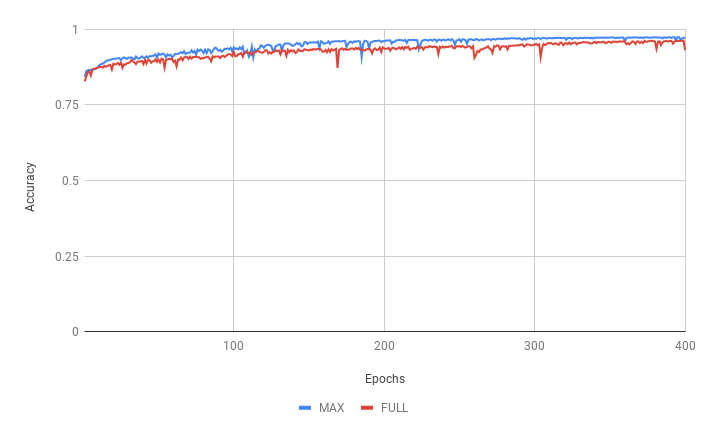
\includegraphics[width=0.48\textwidth]{figures/val_acc.png}
  \caption{Validation accuracy}
  \label{fig:val_accuracy}
\end{figure}

Figure \ref{fig:val_loss} shows the loss behaviour for both networks. Once SLO had the better accuracy than ALO, the loss of was expected smaller, as shown in Figure \ref{fig:val_loss}.

\begin{figure}
  \centering
  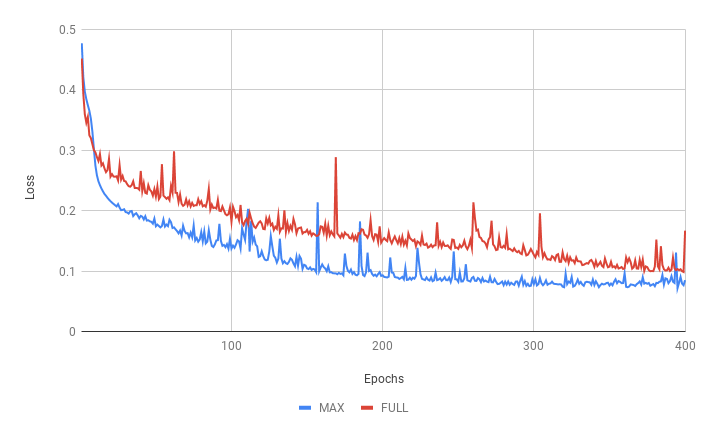
\includegraphics[width=0.48\textwidth]{figures/val_loss.png}
  \caption{Validation loss}
  \label{fig:val_loss}
\end{figure}

For performance comparison, we provide Figure \ref{fig:train_time} and \ref{fig:fps}. Figure \ref{fig:train_time} shows that average time to process SLO network is 12.2\% smaller than ALO network. Figure \ref{fig:fps} shows that SLO can process 33.60 images per second in training time, while ALO process 29.48 images per second.

\begin{figure}
  \centering
  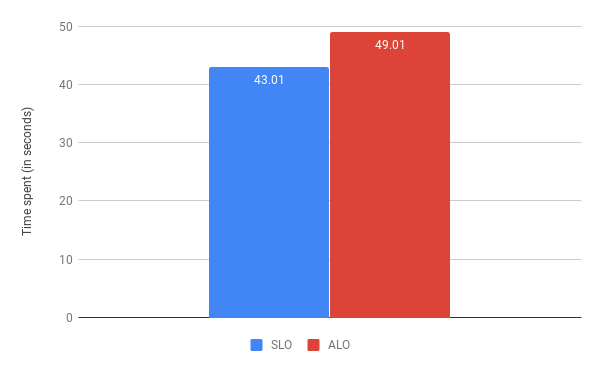
\includegraphics[width=0.48\textwidth]{figures/train_time.png}
  \caption{Average training time}
  \label{fig:train_time}
\end{figure}

\begin{figure}
  \centering
  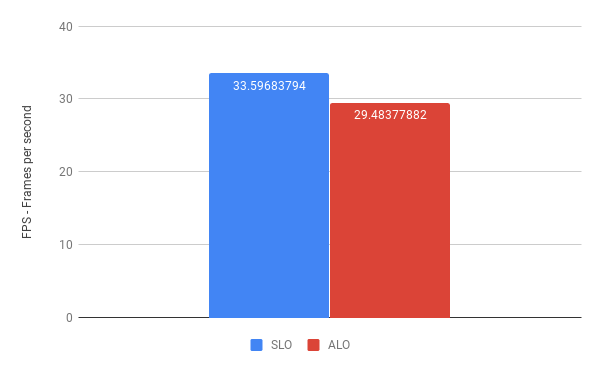
\includegraphics[width=0.48\textwidth]{figures/fps.png}
  \caption{Frames per second}
  \label{fig:fps}
\end{figure}

Once the experiments described above does not reached the best value, we kept training the network for more epochs, in a new test. For SLO network the training, we trained for 2000 epochs using the parameters defined in Section \ref{sec:experimental_setup}. The best accuracy achieve after the training procedures was 0.98080.

ALO network was trained using diferent parameters. Once this network requires less carefully parameters, we defined learning rate as 1e-4, decay as 1e-6 and we used Nesterov optimization. We trained the network util overfitting and get the best value for the validation set. It was necessary 46 epochs to achieve the best accuracy value of 0.98225. Some epochs were close to this values but many ones were smaller, with values closes to 0.86 accuracy.

After the training procedure, we create a post processing step to reduce possible noises in results proposition. For this, we used the mathematical morfology operation of Opening. This procedure removes small noises that could exists in the images, affecting the quality of the results.

We defined a set of kernels with the sizes of $5 \times 5$, $7 \times 7$, $9 \times 9$, $11 \times 11$ and $13 \times 1$ applied in the images to reduce different sizes of noises.

\begin{table}
  \begin{tabular}{{c}{c}{c}{c}{c}{c}{c}}
  
  \multicolumn{7}{l}{Stage Layer Outputs - Without Matematical Morfology} \\
  \hline 
    Category & MaxF & AP & PRE & REC & FPR & FNR \\
  \hline
    \textit{um\_road} & 96.92\% & 87.36\% & 94.47\% & 99.49\% & 1.13\% & 0.51\% \\
    \textit{umm\_road} & 97.57\% & 89.44\% & 96.05\% & 99.15\% & 1.24\% & 0.85\% \\
    \textit{uu\_road} & 95.16\% & 85.73\% & 92.94\% & 97.49\% & 1.16\% & 2.51\% \\
  \hline
  \multicolumn{7}{c}{} \\
  
  \multicolumn{7}{l}{Stage Layer Outputs - With Matematical Morfology} \\
  \hline 	
    Category & MaxF & AP & PRE & REC & FPR & FNR \\
  \hline
    \textit{um\_road} & 97.01\% & 87.68\% & 94.83\% & 99.30\% & 1.05\% & 0.70\% \\
    \textit{umm\_road} & 97.61\% & 89.67\% & 96.30\% & 98.97\% & 1.16\% & 1.03\% \\
    \textit{uu\_road} & 95.42\% & 86.48\% & 93.77\% & 97.13\% & 1.01\% & 2.87\% \\
  \hline
  \multicolumn{7}{c}{} \\
  
  \multicolumn{7}{l}{All Layers Outputs - Without Matematical Morfology} \\
  \hline 	
    Category & MaxF & AP & PRE & REC & FPR & FNR \\
  \hline
    \textit{um\_road} & 96.39\% & 86.81\% & 93.87\% & 99.05\% & 1.25\% & 0.95\% \\
    \textit{umm\_road} & 97.05\% & 88.83\% & 95.37\% & 98.78\% & 1.46\% & 1.22\% \\
    \textit{uu\_road} & 94.70\% & 84.87\% & 92.00\% & 97.56\% & 1.33\% & 2.44\% \\
  \hline
  \multicolumn{7}{c}{} \\
  
  \multicolumn{7}{l}{All Layers Outputs - With Matematical Morfology} \\
  \hline 	
    Category & MaxF & AP & PRE & REC & FPR & FNR \\
  \hline
    \textit{um\_road} & 96.65\% & 87.51\% & 94.64\% & 98.74\% & 1.08\% & 1.26\% \\
    \textit{umm\_road} & 97.21\% & 89.31\% & 95.90\% & 98.56\% & 1.29\% & 1.44\% \\
    \textit{uu\_road} & 95.20\% & 86.15\% & 93.40\% & 97.08\% & 1.08\% & 2.92\% \\
  \hline
  
  \end{tabular}
  \caption{KITTI benchmark evaluation results for in each category \protect\footnotemark}
  \label{table:max_without_morf}
\end{table}

\footnotetext{Table abbreviations: \textit{MaxF}: Maximum F1-measure, \textit{AP}: Average precision, \textit{PRE}: Precision, \textit{REC}: Recall, \textit{FPR}: False Positive Rate, \textit{FNR}: False Negative Rate}

\begin{comment}
HED
Closing for i in range(3, 8, 1):


\end{comment}

\subsection{Qualitative analysis}

In training evaluation, it was noticed that the network was more stable, and we can set bigger learning rates parameters ($1 \times 10^3$). Also, we can use different optimizers and Nesterov Optimization \cite{Nesterov:1983wy}.

